%!TEX root = ../dokumentation.tex

\chapter{Grundlagen eines Netzwerks}



Ein Bussystem ist ein System, bei dem mehrere Teilnehmer über einen gemeinsamen Übertragungsweg verbunden sind und darüber Daten übertragen.
Ein Teilnehmer kann Daten senden oder empfangen, ohne direkt in die Übertragung der anderen Teilnehmer einzugreifen.


\section{Klassifizierung und Überblick von Bussystemen}
Bussysteme können grundsätzlich in vier Klassen unterteilt werden, die jeweils einen Unterschiedlichen Anwendungszweck erfüllen.
\begin{figure}[!htbp]
    \centering
    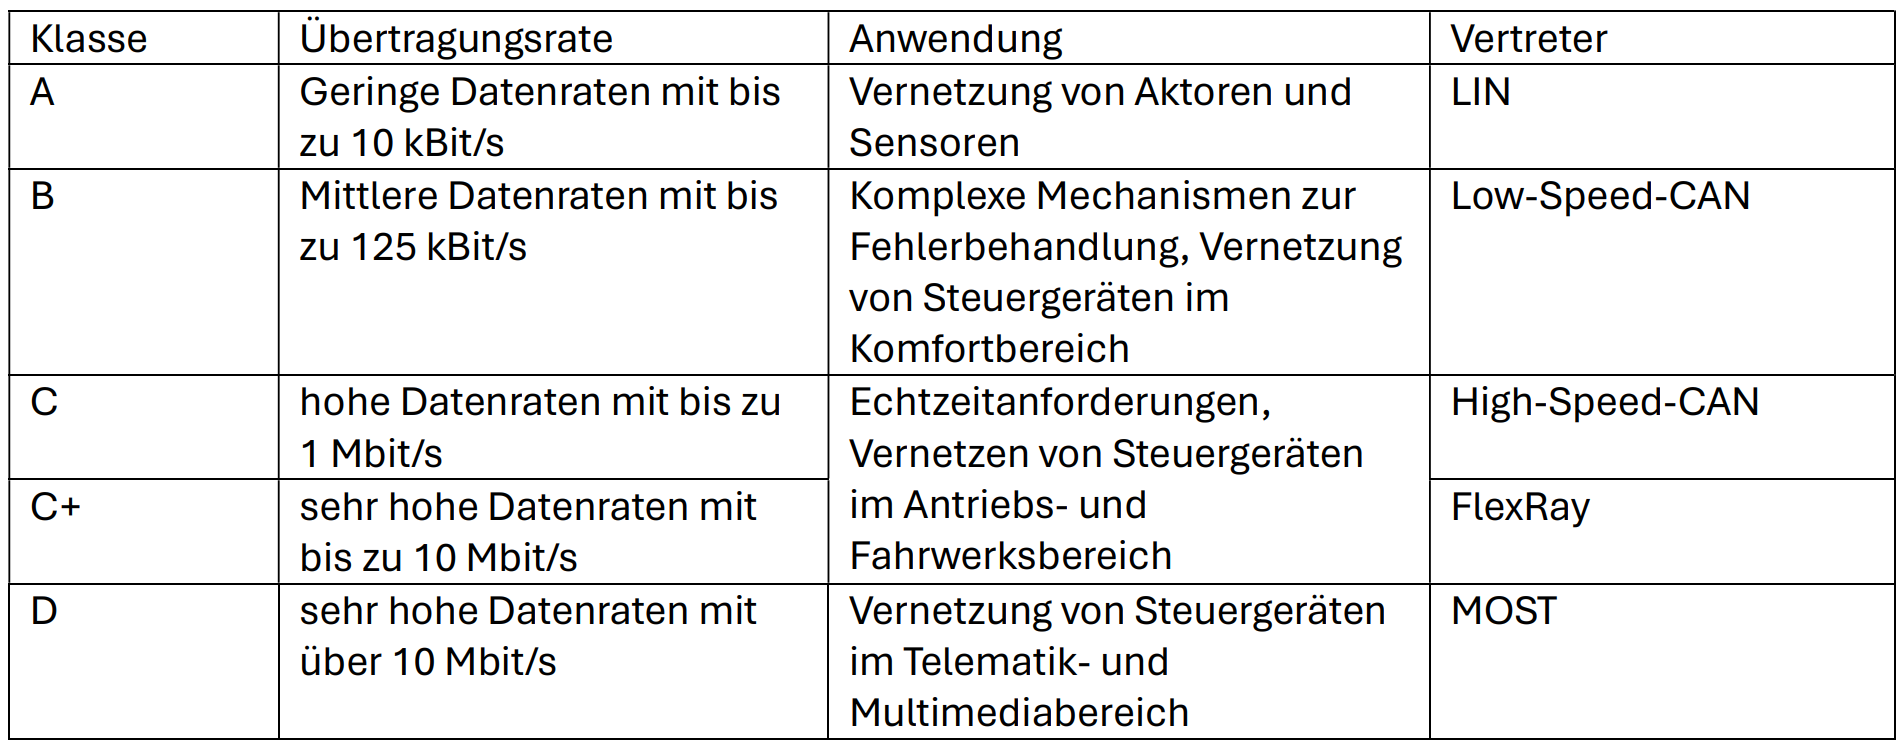
\includegraphics[width=1\linewidth]{own/Grundlagen/Busarten_Eigen.png}
    \caption{Tabelle Busarten, überarbeitet, Quelle: \cite{BAA2011, S.82}}
    \label{fig:Busarten}
\end{figure}
    
\section{Einsatzgebiete im KFZ}
Elektronische Anwendungen sind aus dem heutigen Automobil nicht mehr wegzudenken, weshalb es nötig ist, die unterschiedlichen Steuergeräte untereinander zu vernetzen, was die Notwendigkeit für ein Bussystem bringt.
Grundsätzlich ist die Vernetzung von Autos in vier Hauptbereiche mit unterschiedlichen Anforderungen unterteilt.
Die ersten zwei Hauptbereiche, der Antriebsstrang und das Chassis, beinhalten Echtzeitanwendungen, die hohe Anforderungen an die Leistungsfähigkeit benötigen, da die Zyklenzeiten des Busses oft im Bereich von wenigen Millisekunden liegen.
Diese werden der Klasse C zugewiesen und es wird hauptsächlich High-Speed-\acused{CAN}\ac{CAN} mit 500.000 Bitsendungen pro Sekunde (500k Baud) eingesetzt, da die Klasse C zusätzlich zu den recht hohen Datenraten auch sehr hohe Anforderungen an die Fehlertoleranz hat.
Beispiele für Echtzeitanwendungen wären das Motormanagement, \ac{ABS} oder \ac{ESP}, da diese Systeme unterschiedliche Daten aus verschiedenen Sensoren und Steuergeräten zuverlässig verarbeiten müssen.
Ein weiterer Hauptbereich ist der Innenraum, der in den Bereich der Multiplex-Anwendung fällt.
Bei einer Multiplex-Anwendung werden verschiedene Signale über eine Leitung übertragen, was vor allem für die Steuerung von Karosserieelementen (z.B. Anzeigen, Beleuchtung) und Komfortelementen (z.B. Sitzverstellung, Klimaregelung) nützlich ist.
Diese werden meist zur Klasse B oder teilweise auch zur Klasse A zugeordnet. Diese Busse besitzen im Vergleich zur Klasse C geringere Anforderungen an die Datenübertragungsrate und Fehlererkennung, da damit keine kritischen Anwendungen gesteuert werden.
Der vierte Hauptbereich ist das Infotainment, was in der Telematik beinhaltet wird und von Bussen der Klasse D angesteuert wird.

\begin{figure}[!htbp]
    \centering
    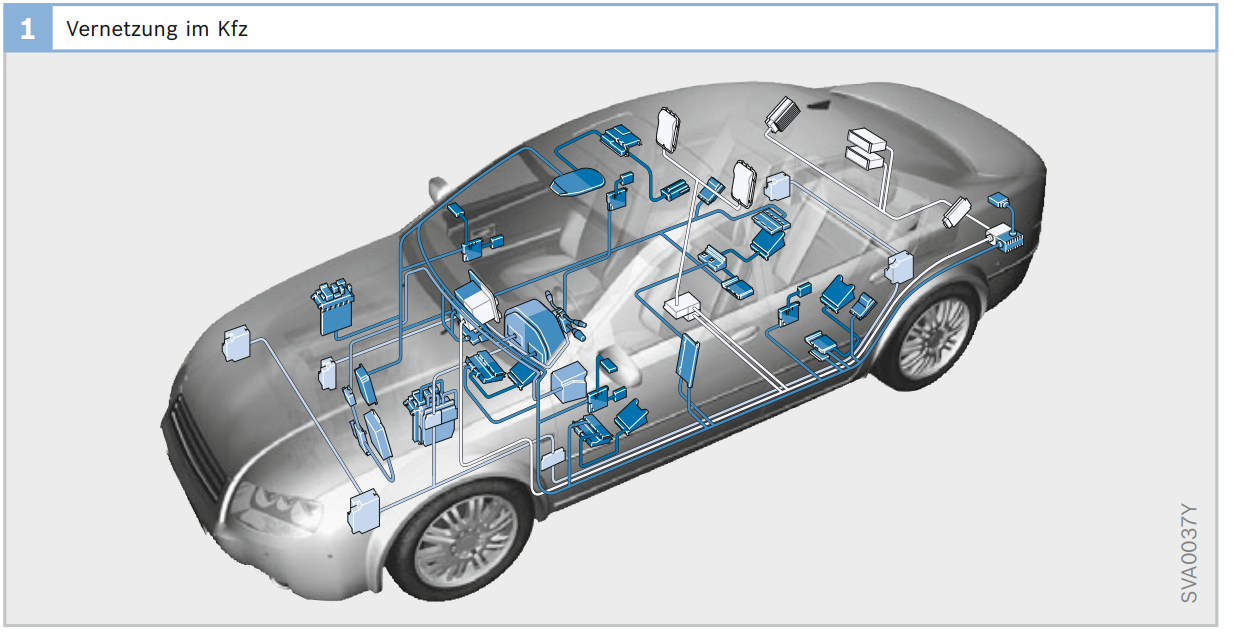
\includegraphics[width=1\linewidth]{own/Grundlagen/VernetzungImKFZ_BBA82.png}
    \caption{Grafik Vernetzung im \ac{Kfz}, Quelle: \cite{BAA2011, S.85}}
    \label{fig:VernetzungImKFZ}
\end{figure}

\section{Anforderungen an ein Bussystem}
    \subsection{Datenübertragungsrate}
    Die benötigte Datenübertragungsrate ist stark vom Einsatzweck abhängig.
    Ein Schalter zum Einschalten eines Lichts braucht wenige Bit und eine geringe Übertragungsrate, während die Übertragung einer Geschwindigkeit mit einer sehr hohen Genauigkeit und Updaterate eine deutlich höhere Datenübertragungsrate benötigt.
    Die Datenübertragungsrate wird meist in Bit/s oder einer Vielfachen davon angegeben (z.B. kBit/s, Mbit/s). 

    \subsection{Störsicherheit}
    Ein Ideales Bussystem ist komplett störsicher.
    Dies ist in der Praxis aber unmöglich zu erreichen, weshalb verschiedene Maßnahmen getroffen werden müssen, um eine Sichere Datenübertragung für z.B. die Motorsteuerung oder das \ac{ABS} zu erreichen.
    Zur Erkennung von Übertragungsfehlern werden in das Netzwerkprotokoll verschiedene Sicherheitsmechanismen eingebaut.
    Ein beliebtes und einfaches und Mittel ist das Paritätsbit.
    Mit dem Paritätsbit wird für den zu übertragenen Datenblock (in Bit) geprüft, ob die Summe der Bits gerade oder ungerade ist.
    Dies wird auf Senderseite berechnet und der Nachricht angehängt, damit die Empfängerseite dies auch berechnen kann und mit dem empfangenen Wert vergleichen kann.
    Dasselbe Verfahren wird bei der Checksummenprüfung verwendet, wobei hier nicht nach der Parität geprüft wird, sondern aus den einzelnen Datenbits eine Prüfsumme berechnet wird.
    Diese Prüfsummenberechnung kann sich nach Protokoll und Anwendung unterscheiden.

    \subsection{Echtzeitfähigkeit}
    Die Echtzeitfähigkeit garantiert, dass die Berechnung und Übertragung von Daten innerhalb eines festgelegen Zeitintervalls stattfinden.
    Das erforderte Zeitintervall hängt auch wieder vom Anwendungszweck ab, weshalb es verschiedene Anforderungen an das Echtzeitverhalten gibt.
    Bei einer weichen Echtzeitanforderung hält ein System die vorgegebene Zeitvorgabe in der Regel ein, wobei diese gelegentlich auch überschritten werden kann, ohne dass dies gravierende Auswirkungen für das System hat.
    Im Gegensatz dazu steht die harte Echtzeitanforderung, bei der die vorgegebene Zeitvorgabe strikt eingehalten werden muss, da bei der Überschreitung dieser, die Daten nicht mehr verwendbar sind.
    Dies kann bei sicherheitsrelevanten Systemen, wie z.B. \ac{ABS} oder der Motorsteuerung, zu schweren Problemen führen.
    Wenn ein Steuergerät Daten von einem anderen Steuergerät benötigt, muss das Bussystem die benötigte Datenübertragungsrate und das vorgeschriebene Zeitintervall einhalten, damit das Bussystem der gestellten Echtzeitanforderung genügt.

    \subsection{Netzknotenanzahl und Kopplung von Netzwerken}
    Ein Netzknoten ist ein Teilnehmer an der Buskommunikation und die maximale Netzknotenanzahl gibt die maximale Anzahl der einzubindenden Netzknoten an, welche für verschiedene Anwendungszwecke unterschiedlich ist. 
    \\
    Ein Gateway ist ein Rechner, der die Möglichkeit verschafft zwischen unterschiedlichen Protokollen zu kommunizieren.
    Dieser liest die Daten aus einem Protokoll ein, puffert diese und sendet sie mit einem anderen Protokoll auf einem anderen Subnetz.
    \\
    Oft kommen auch mehrere gleiche Bussysteme für unterschiedliche Anwendungszwecke zum Einsatz, die miteinander kommunizieren müssen.
    Dies kann über mehrere verteilte Gateways geschehen oder über einen Zentralen Gateway.
    Der Trend geht allerdings immer mehr in Richtung eines zentralen Gateway, da man damit Kosten, durch die weniger verbauten Steuergeräte, sparen kann.

    \begin{figure}[!htbp]
        \centering
        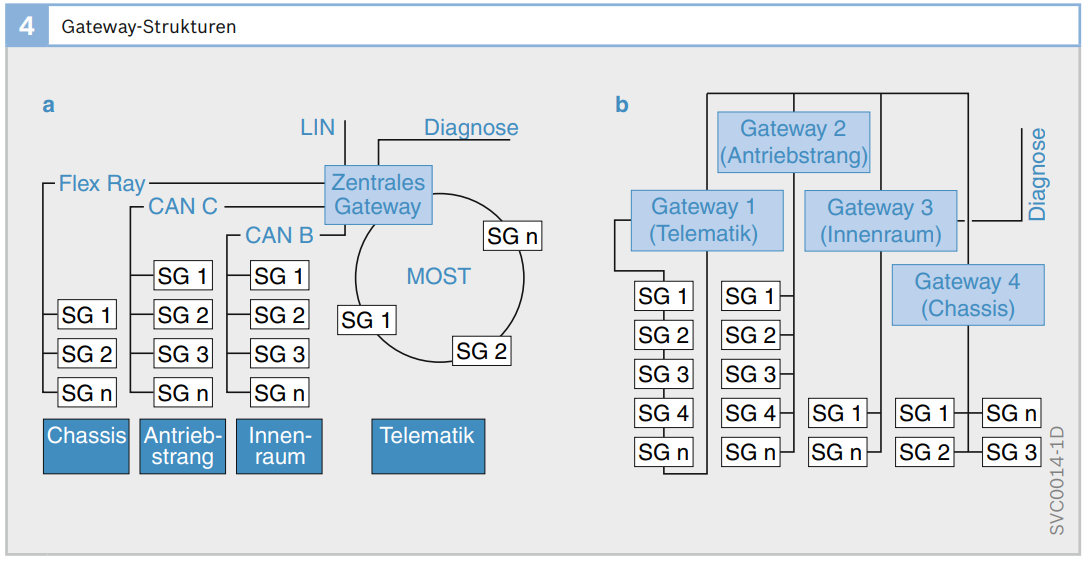
\includegraphics[width=0.7\linewidth]{own/Grundlagen/KopplungUndGatewayStruktur_BBA87.png}
        \caption{Grafik Gateway-Strukturen, Quelle: \cite{BAA2011, S.87}}
        \label{fig:GatewayStrukuren}
    \end{figure}
    
\section{Grundlagen}

    \subsection{Topologien}
Eine Topologie beschreibt den Aufbau eines Netzwerks.
Hier werden nur die Bustopologie und die Sterntopologie beschrieben, da diese für das Bussystem in Automobilen hauptsächlich verwendet und kombiniert werden.
Es gibt allerdings noch unzählige weitere Topologien.
    \subsubsection{Bustopologie}
    Die Bustopologie benötigt keine zentrale Steuereinheit, um eine Kommunikation durchzuführen.
    Es werden alle Netzwerkknoten an einen zentralen Bus angeschlossen, über den die Kommunikation stattfindet.
    Dies hat den Vorteil, dass weitere Netzknoten einfach und kostengünstig hinzugefügt werden können und ein Netzknoten ausfallen kann, ohne die Funktionstüchtigkeit der anderen Teilnehmer zu beeinträchtigen.
    
    \subsubsection{Sterntopologie}
    Bei der Sterntopologie gibt es ein zentrales Koppelelement, an dem mehrere Subnetze oder Steuergeräte angeschlossen sind.
    Dies schafft eine höhere Anpassungsfähigkeit beim Vernetzen, durch z.B. unterschiedlich eingesetzte Protokolle.
    Allerdings muss das Koppelelement alle Nachrichten bearbeiten und weiterleiten.
    Außerdem muss zum Erreichen einer gleichen Signallaufzeit die gleiche Leitungslänge verwendet werden.

    \begin{figure}[!htbp]
        \centering
        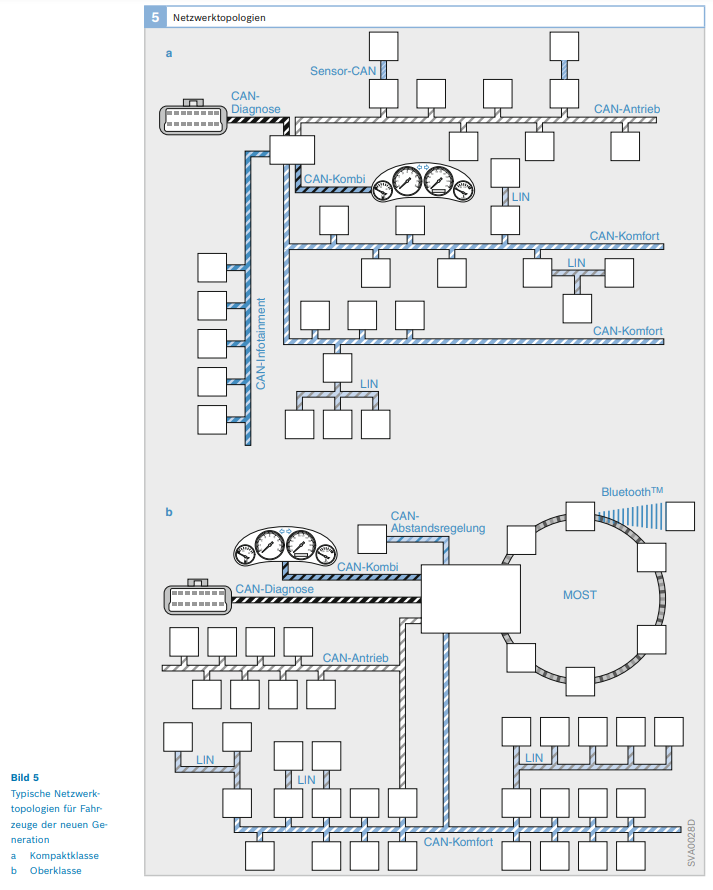
\includegraphics[width=0.5\linewidth]{own/Grundlagen/Netztopologien_BBA88.png}
        \caption{Grafik Netzwerktopologien, Quelle: \cite{BAA2011, S.88}}
        \label{fig:Netzwerktopologien}
    \end{figure}

    \subsection{Adressierung}
    Damit eine Nachricht und deren Informationen bei der Datenübertragung auf einem Bus identifiziert werden kann, erhält sie zusätzlich zum Datenpacket auch eine Information zur Datenübertragung.
    Diese wird genutzt, um sie zu identifizieren und dem richtigen Empfänger zukommen zu lassen.
    Es gibt mehrere Arten der Adressierung, die unterschiedliche Ansätze verfolgen.
    Bei der teilnehmerorientieren Adressierung, erhält die Nachricht als Identifikation eine Knotenadresse und alle anderen Knoten prüfen, ob die gesendete Nachricht die richtige Knotenadresse hat.
    Das nachrichtenorientierte Verfahren arbeitet mit der Adressierung von Nachrichten, wo die zu Knoten, die etwas empfangen, selbst entscheiden, ob sie die Nachricht verarbeiten wollen.
    Dadurch brauchen die Knoten keine Information über die Systemkonfiguration und können unabhängig voneinander arbeiten, zudem können Empfangsstationen ohne Änderungen hinzugefügt werden, was eine sehr hohe Flexibilität bietet.
    Beim Übertragungsorientierten Verfahren, welches gerne mit den oben genannten Verfahren kombiniert wird, erfolgt die Adressierung mit Übertragungsmerkmalen wie z.B. einem Zeitfenster, in dem eine Nachricht gesendet wird. 

    \subsection{Zugriffsarten auf einen Bus}
    Um eine Nachricht auf einem Bus zu senden, muss der Knoten auf den Bus zugreifen können.
    Die Regelung davon, geschieht entweder mit einem vorhersehbaren Verfahren (z.B. bestimmte Zeitpunkte für jeden Knoten) oder mit einem zufälligen Verfahren, bei dem jeder Knoten bei einem freien Bus probiert eine Nachricht zu senden.
    Desweitern kann man zwischen Time Division Multiple Access (in diesem Referat nicht behandelt), Master-Slave und Multimaster unterschieden werden.
    \subsubsection{Master-Slave}
    Beim Master-Slave Verfahren gibt ein Master den Zeitpunkt und die Häufigkeit der einzelnen Sendungen der Slaves an.
    Der Slave antwortet nur, wenn er von einem Master angesprochen wird.
    Manche Master-Slave Protokolle erlauben es allerdings, dass sich der Slave beim Master mit einer Sendungsbitte meldet. 
    
    \subsubsection{Multimaster}
    Im Gegensatz zum Master-Slave Verfahren sind beim Multimaster Verfahren alle Knoten Master und dürfen alle selbstständig und unkontrolliert auf einen Bus zugreifen.
    Deshalb muss es eine Möglichkeit zur Kollisionserkennung geben, die dann z.B. eine Nachricht priorisiert und die andere Nachricht verzögert.

    \subsection{Steuermechanismen}
    Wann eine Nachricht gesendet wird, kann anhand von zwei Verfahren determiniert werden, die nach unterschiedlichen Prinzipien arbeiten.
    
    \subsubsection{Ereignissteuerung}
    Eine Nachricht wird bei der Ereignissteuerung dann übertragen, wenn dies durch ein Ereignis gefordert wird.
    Dies bietet die Vorteile, dass man eine große Reaktionsfähigkeit auf asynchrone Ereignisse hat, einfach neue Knoten nachrüsten kann.
    Außerdem wird das Netzwerk nicht mit unnötigen Übertragungen belastet.
    Allerdings ist diese Art der Ereignissteuerung nicht deterministisch, weshalb man nicht nachweisen kann, wann eine Nachricht gesendet wurde. 
    

    \begin{figure}
        \centering
        \begin{minipage}{.5\textwidth}
          \centering
          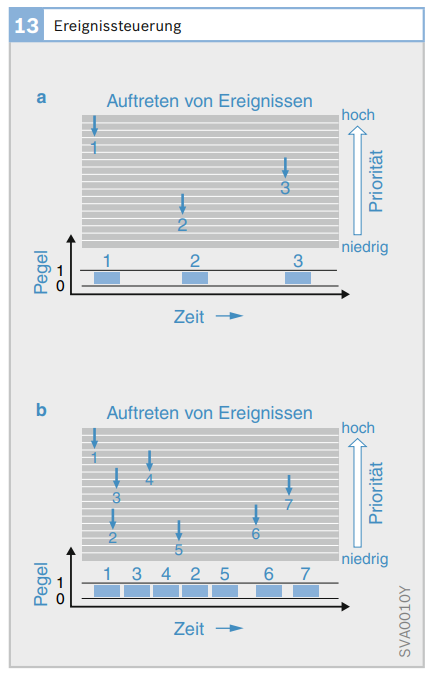
\includegraphics[width=0.7\linewidth]{own/Grundlagen/Ereignissteuerung_BBA78.png}
          \caption{Grafik Ereignissteuerung, Quelle: \cite{BAA2011, S.78}}
            \label{fig:Ereignissteuerung}
        \end{minipage}%
        \begin{minipage}{.5\textwidth}
          \centering
          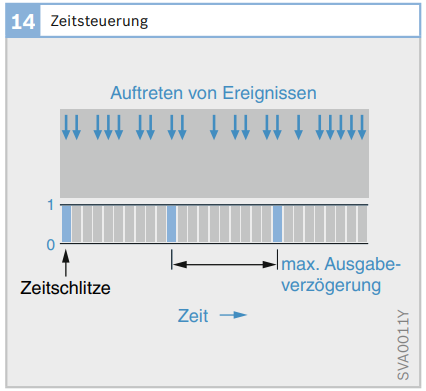
\includegraphics[width=0.7\linewidth]{own/Grundlagen/Zeitsteuerung_BBA80.png}
          \caption{Grafik Zeitsteuerung, Quelle: \cite{BAA2011, S.80}}
        \label{fig:Zeitsteuerung}
        \end{minipage}
        \end{figure}


    %\begin{figure}[!htbp]
    %    \centering
    %    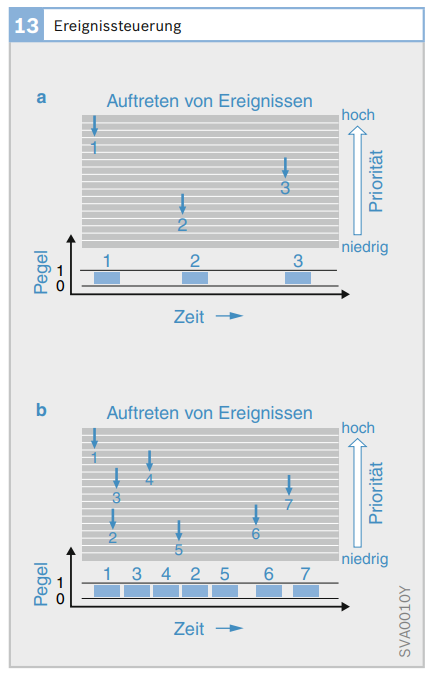
\includegraphics[width=0.5\linewidth]{own/Grundlagen/Ereignissteuerung_BBA78.png}
    %    \caption{Grafik Ereignissteuerung, Quelle: \cite{BAA2011, S.78}}
    %    \label{fig:Ereignissteuerung}
    %\end{figure}

    \subsubsection{Zeitsteuerung}
    Bei der Zeitsteuerung ist dies allerdings ohne Probleme möglich, da die Nachrichten nach einem Netzwerkplan, ohne Kollision, hintereinander abgearbeitet werden.
    Damit ist die Zeitliche Aktualität einer Nachricht immer bestimmt und eine Nachricht kann nicht unterdrückt werden.
    Hier muss die Kapazität für eine Netzerweiterung allerdings angepasst werden und es gibt nur eine geringe Reaktionsfähigkeit auf asynchrone Ereignisse.
    Die Echtzeitanforderung kann trotz Zeitsteuerung bei einem schnellen System auch erreicht werden. 
    %\begin{figure}[!htbp]
    %    \centering
    %    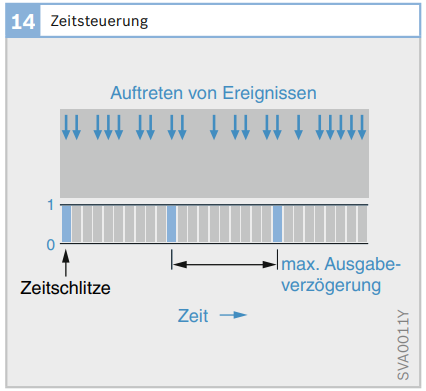
\includegraphics[width=0.5\linewidth]{own/Grundlagen/Zeitsteuerung_BBA80.png}
    %    \caption{Grafik Zeitsteuerung, Quelle: \cite{BAA2011, S.80}}
    %    \label{fig:Zeitsteuerung}
    %\end{figure}

    \subsection{Quantisierung}
    Da in einem Kraftfahrzeug viele verschiedene Signale verarbeitet werden, müssen diese in das richtige Format gebraucht werden.
    Schalterzustände können \ac{z.B.} einfach durch ein Bit dargestellt werden, während \ac{z.B.} Temperaturen oder Spannungen erst noch quantisiert werden müssen.
    Beim Quantisieren wandelt man die Werte von kontinuierlichen und unendlichen Werten in diskrete Werte um.
    Allerdings muss, um die Wertegleichheit der Systeme aufrecht zu erhalten, in allen Systemen gleich zwischen binär und physikalischer Form umgerechnet werden. 

    